\documentclass[a4paper,12pt]{article}
\usepackage[russian]{babel}
\usepackage[T2A]{fontenc}
\usepackage[utf8]{inputenc}
\usepackage{geometry}
\usepackage{amsmath}
\usepackage{graphicx}
\usepackage{cancel}
\usepackage{float} 
\usepackage{xcolor}
\usepackage{array}
\usepackage{caption}
\usepackage{booktabs}
\usepackage{amssymb}
\usepackage{subcaption}
\usepackage{pgfplots}
\pgfplotsset{compat=1.18}
\usetikzlibrary{arrows.meta, matrix}
\usepackage{capt-of}
\usepackage{multirow}
\usepackage[siunitx]{circuitikz}
\usepackage[bottom]{footmisc}
\usepackage{tcolorbox}
\usepackage{nicematrix}
\usepackage{tikz}
\usetikzlibrary{positioning, arrows.meta}

% --- hyperref ОДИН РАЗ ---
\usepackage{hyperref}
\hypersetup{linktoc=page}
\hypersetup{
	colorlinks=true,
	linkcolor=red,
	citecolor=red,
	urlcolor=red,
	filecolor=red,
}

% --- Содержание ---
\usepackage{tocloft}
\usepackage{etoolbox}
\usepackage{hyperref}
\hypersetup{
	colorlinks=true,
	linkcolor=red,
	citecolor=red,
	urlcolor=red,
}

% Патчим \tableofcontents: текст строк — без ссылок и чёрный
% Это делается через замену \contentsline внутри TOC
\preto\tableofcontents{%
	\begingroup
	% Переопределяем contentsline так, чтобы текст был чёрным без ссылки,
	% а номер страницы — красной ссылкой
	\renewcommand{\contentsline}[4]{%
		\ifnum\pdfstrcmp{##1}{section}=0
		\vskip 4pt{\normalfont\color{black}##2}\nobreak\hfill
		{\normalfont\color{red}\hyperlink{##4}{##3}}\par
		\else\ifnum\pdfstrcmp{##1}{subsection}=0
		\vskip 2pt\hspace{1.5em}{\normalfont\color{black}##2}\nobreak\hfill
		{\normalfont\color{red}\hyperlink{##4}{##3}}\par
		\else
		\vskip 1pt\hspace{3em}{\normalfont\color{black}##2}\nobreak\hfill
		{\normalfont\color{red}\hyperlink{##4}{##3}}\par
		\fi\fi
	}%
}
\appto\tableofcontents{\endgroup}

% tocloft — только для отступов, без переопределения шрифтов
\usepackage{tocloft}

% --- Листинги ---
\usepackage{listings}

\definecolor{codebg}{RGB}{250,250,252}
\definecolor{linenumcolor}{RGB}{150,150,170}
\definecolor{mathblue}{RGB}{30,100,200}
\definecolor{mathorange}{RGB}{200,100,20}
\definecolor{matlabblue}{RGB}{0,0,200}
\definecolor{matlabgreen}{RGB}{30,130,30}
\definecolor{matlaborange}{RGB}{200,80,0}


\lstdefinestyle{matlab}{
	language=Matlab,
	basicstyle=\ttfamily\small,
	keywordstyle=\color{matlabblue}\bfseries,
	commentstyle=\color{matlabgreen}\itshape,
	stringstyle=\color{matlaborange},
	numberstyle=\tiny\color{linenumcolor},
	numbers=left,
	numbersep=10pt,
	backgroundcolor=\color{codebg},
	frame=single,
	frameround=tttt,
	framesep=4pt,
	rulecolor=\color{matlabblue!30},
	breaklines=true,
	tabsize=4,
	showstringspaces=false,
	captionpos=b,
	xleftmargin=15pt,
	xrightmargin=5pt,
	escapeinside={\%*}{*)},
	morekeywords={cvx_begin,cvx_end,sdp,variable,minimize,maximize},
}

\lstset{style=matlab}

\renewcommand{\lstlistingname}{Листинг}
\DeclareCaptionFormat{redlisting}{#1\textcolor{red}{#2}#3}
\captionsetup[lstlisting]{format=redlisting}

\geometry{left=1.5cm, right=2cm, bottom=2cm, top=2cm}
\captionsetup[figure]{name=Рисунок}
\captionsetup[table]{name=Таблица}
\captionsetup{labelsep=endash}

\newcommand{\figwidth}{0.6\textwidth}

\begin{document}
	
	\begin{titlepage}
		\centering
		
		\vspace*{0.5cm}
		{\small
			Министерство науки и высшего образования Российской Федерации\\[2pt]
			Федеральное государственное автономное образовательное учреждение\\
			высшего образования\\[2pt]
			\textbf{«Национальный исследовательский университет ИТМО»}\\
		}
		
		\vspace{0.8cm}
		\hrule height 0.8pt
		\vspace{0.3cm}
		
		{\large Факультет систем управления и робототехники}
		
		\vspace{0.3cm}
		\hrule height 0.4pt
		\vspace{2.5cm}
		
		{\Huge\bfseries ОТЧЁТ}\\[0.4cm]
		{\LARGE\bfseries о лабораторной работе}\\[0.8cm]
		
		\begin{tcolorbox}[
			colback=gray!4,
			colframe=gray!10,
			boxrule=0.8pt,
			arc=4pt,
			left=12pt, right=12pt, top=8pt, bottom=8pt
			]
			\centering
			{\large По дисциплине:\\[4pt]}
			{\large\bfseries «Теория автоматического управления»}\\[10pt]
			{\large Тема:\\[4pt]}
			{\large\bfseries «Управление многоканальной системой»} \\[10pt]
			{\large Поток: 1.1.3 \( \) Вариант: 25}
		\end{tcolorbox}
		
		\vspace{3cm}
		
		\begin{minipage}{0.45\textwidth}
			\raggedright
			{\large\bfseries Студент:}\\[4pt]
			Охрименко Е.\,Д.\\
		\end{minipage}
		\hfill
		\begin{minipage}{0.45\textwidth}
			\raggedleft
			{\large\bfseries Преподаватель:}\\[4pt]
			Пашенко А.\,В.\\
		\end{minipage}
		
		\vfill
		\vspace{0.4cm}
		{\large Санкт-Петербург, 2026}
	\end{titlepage}
	
	\newpage
	\tableofcontents
	
	\newpage \section{Исследование свойств многоканальной системы}\label{sec:1}
	
	В соответствии с вариантом рассмотрю систему:
	
		\begin{equation}
		\begin{cases}
			\dot{x} = Ax + Bu \\
			y = C x
		\end{cases}
		\label{sys}
	\end{equation}
	
	где:
	
	\[
	A = \begin{bmatrix} 
		0 & 1  \\ 
		-3 & 4 
	\end{bmatrix} \qquad
	B = \begin{bmatrix} 
		3 & -5  \\ 
		2 & 0 
	\end{bmatrix}\qquad
	C = \begin{bmatrix} 
		4 & 1  \\ 
		-2 & 0 
	\end{bmatrix}
	\]

	
	Требуется:
	\begin{enumerate}
		\item Найти собственные числа матрицы $A$.
		
		\item Определить передаточную матрицу $W(s) = C(sI - A)^{-1}B$, найти полюса и нули системы, сравнить с собственными числами $A$.
		
		\item Исследовать систему на:
		\begin{itemize}
			\item управляемость по состоянию и стабилизируемость;
			\item наблюдаемость и обнаруживаемость;
			\item управляемость по выходу.
		\end{itemize}
		
		\item Вывести аналитические выражения для весовой $g(t)$ и переходной $h(t)$ характеристик, построить их графики.
		
		\item Вывести аналитические выражения для АЧХ, ФЧХ, ЛАЧХ и ЛФЧХ, построить их графики.
		
		\item Сделать выводы.
	\end{enumerate}
	
	\hrule \newpage \subsection{Анализ собственных чисел матрицы системы}
	
	Используя характеристическое уравнение:
	
	\[
	\det(\lambda I - A) = \det\begin{bmatrix}
		\lambda & -1 \\
		3 & \lambda - 4
	\end{bmatrix} = \lambda(\lambda - 4) + 3 = \lambda^2 - 4\lambda + 3 = 0
	\]
	
	Найду корни матрицы системы:
	\[
	\lambda_{1,2} = \frac{4 \pm \sqrt{16 - 12}}{2} = \{1, 3\}
	\]
	
	\subsection{Передаточная матрица многоканальной системы}
	
	Найду предаточную матрицу системы (листинг~\ref{lst:W1}):
	
	\[
	W(s) = C(sI - A)^{-1}B = 
	\frac{1}{s^2 - 4s + 3}
	\begin{bmatrix}
		14s - 49 & -20s + 95 \\
		-6s + 20 & 10s - 40
	\end{bmatrix}
	\]
	
	Знаменатель:
	
	\[
	s^2 - 4s + 3 = (s - 1)(s - 3)
	\]
	
	Полюса системы: $s_1 = 1$, $s_2 = 3$, совпадают с собственными числами матрицы $A$.
	
	
	Определитель передаточной матрицы (листинг~\ref{lst:detW1}):
	
	\[
	\det W(s) = \frac{20}{s^2 - 4s + 3} = \frac{20}{(s - 1)(s - 3)}
	\]
	
	Числитель определителя не обращается в ноль ни при каких $s$, следовательно, передаточная матрица не имеет нулей.
	
	\subsection{Управляемость и наблюдаемость системы}
	
	Исследую систему по пройденным на курсе критериям.
	
	
	\begin{enumerate}
		\item Построю матрицу управляемости (листинг~\ref{lst:Co1}):
		
		\[
		\mathcal{C} = \begin{bmatrix} B & AB \end{bmatrix} = 
		\begin{bmatrix}
			3 & -5 & 2 & 0 \\
			2 & 0 & -1 & 15
		\end{bmatrix}
		\]
		
		\[
		\text{rank}(\mathcal{C}) = 2
		\]
		
		Следовательно, система полностью управляема по состоянию, а значит  стабилизируема.
		
		
		\item Матрица наблюдаемости (листинг~\ref{lst:Ob1}):
		
		\[
		\mathcal{O} = \begin{bmatrix} C \\ CA \end{bmatrix} = 
		\begin{bmatrix}
			4 & 1 \\
			-2 & 0 \\
			-3 & 8 \\
			0 & -2
		\end{bmatrix}
		\]
		
		\[
		\text{rank}(\mathcal{O}) = 2
		\]
		
		Следовательно, система полностью наблюдаема, а значит, и обнаруживаема.
		
		\item Матрица управляемости по выходу (листинг~\ref{lst:Co_out1}):
		
		\[
		\mathcal{C}_y = \begin{bmatrix} CB & CAB \end{bmatrix} = 
		\begin{bmatrix}
			14 & -20 & 7 & 15 \\
			-6 & 10 & -4 & 0
		\end{bmatrix}.
		\]
		
		\[
		\text{rank}(\mathcal{C}_y) = 2
		\]
		
		Следовательно, система управляема по выходу.
		
	\end{enumerate}
	
	\subsection{Временные характеристики}
	
	
	Весовая характеристика системы (листинг~\ref{lst:g1}):
	
	\[
	g(t) = \mathcal{L}^{-1}\{W(s)\} =
	\begin{bmatrix}
		\dfrac{11}{2}e^{3t} - \dfrac{7}{2}e^{t} & \dfrac{35}{2}e^{3t} - \dfrac{75}{2}e^{t} \\[10pt]
		e^{3t} - 7e^{t} & -5e^{3t} + 15e^{t}
	\end{bmatrix}
	\]
	
	Переходная характеристика системы (листинг~\ref{lst:h1}):
	
	\[
	h(t) = \mathcal{L}^{-1}\left\{\dfrac{W(s)}{s}\right\} =
	\begin{bmatrix}
		\dfrac{35}{2}e^{t} - \dfrac{7}{6}e^{3t} - \dfrac{49}{3} & \dfrac{35}{6}e^{3t} - \dfrac{75}{2}e^{t} + \dfrac{95}{3} \\[10pt]
		\dfrac{1}{3}e^{3t} - 7e^{t} + \dfrac{20}{3} & 15e^{t} - \dfrac{5}{3}e^{3t} - \dfrac{40}{3}
	\end{bmatrix}
	\]
	
	
	Построю графики весовой и переходной характеристик системы.
	
	\begin{figure}[H]
		\centering
		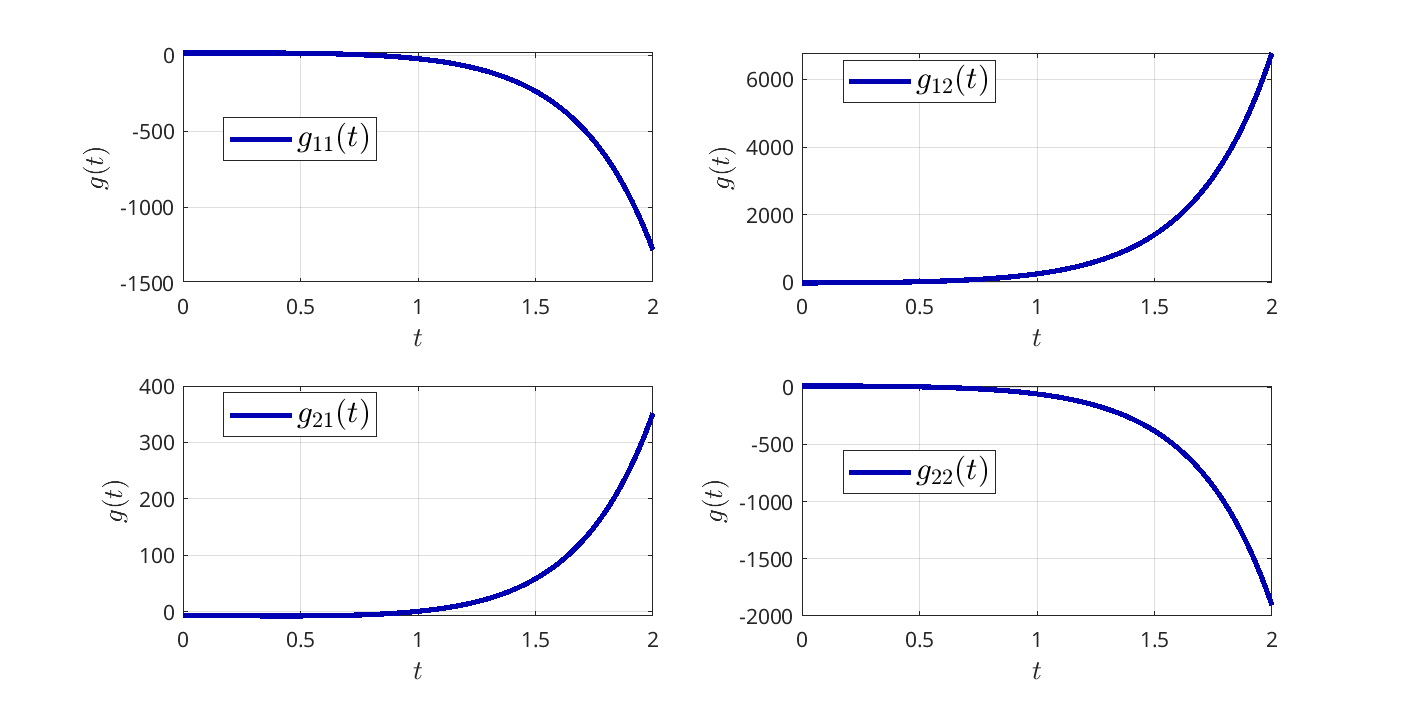
\includegraphics[width=1\textwidth]{../../report/images/task1/g.png}
		\caption{Весовая характеристика $g(t)$}
	\end{figure}
	
	\begin{figure}[H]
		\centering
		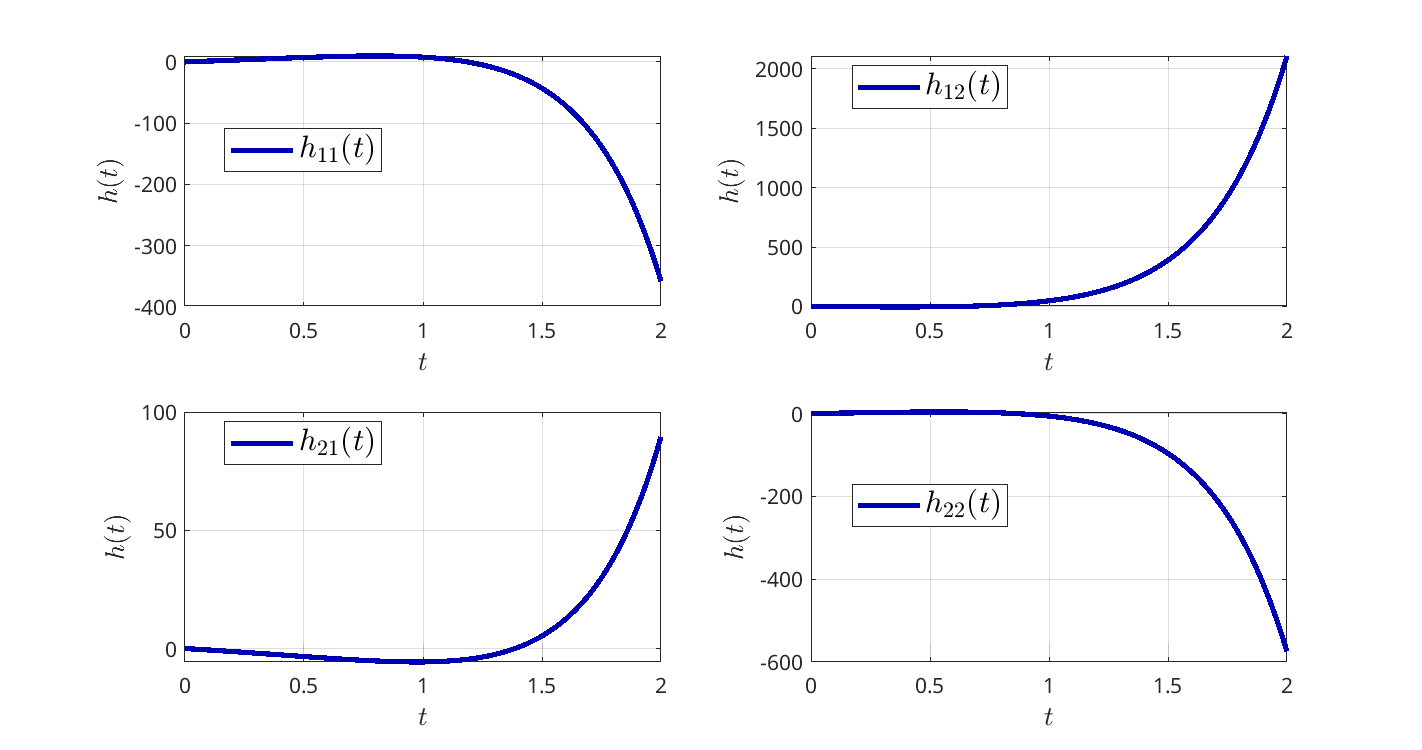
\includegraphics[width=1\textwidth]{../../report/images/task1/h.png}
		\caption{Переходная характеристика $h(t)$}
	\end{figure}
	
	
	\subsection{Частотные характеристики системы}
	
	Для построения частотных характеристик выполним подстановку $s = j\omega$ в передаточную матрицу:
	
	\[
	W(j\omega) = \frac{1}{(j\omega)^2 - 4j\omega + 3}
	\begin{bmatrix}
		14j\omega - 49 & -20j\omega + 95 \\
		-6j\omega + 20 & 10j\omega - 40
	\end{bmatrix}
	\]
	
Амплитудно-частотные характеристики (АЧХ) (листинг~\ref{lst:ach1}):

\[
A(\omega) = |W(j\omega)| =
\begin{bmatrix}
	\dfrac{7|7 - 2j\omega|}{|\omega^2 + 4j\omega - 3|} & \dfrac{5|19 - 4j\omega|}{|\omega^2 + 4j\omega - 3|} \\[10pt]
	\dfrac{2|10 - 3j\omega|}{|\omega^2 + 4j\omega - 3|} & \dfrac{10|4 - j\omega|}{|\omega^2 + 4j\omega - 3|}
\end{bmatrix}
\]

Фазочастотные характеристики (ФЧХ) (листинг~\ref{lst:fch1}):

\[
\varphi(\omega) = \arg W(j\omega) =
\begin{bmatrix}
	\arg\left(-\dfrac{-7 + 2j\omega}{\omega^2 + 4j\omega - 3}\right) & \arg\left(\dfrac{-19 + 4j\omega}{\omega^2 + 4j\omega - 3}\right) \\[10pt]
	\arg\left(\dfrac{-10 + 3j\omega}{\omega^2 + 4j\omega - 3}\right) & \arg\left(-\dfrac{-4 + j\omega}{\omega^2 + 4j\omega - 3}\right)
\end{bmatrix}.
\]
	
	
	Построю графики АЧХ, ЛАЧХ, ФЧХ, ЛФЧХ.
	
	\begin{figure}[H]
		\centering
		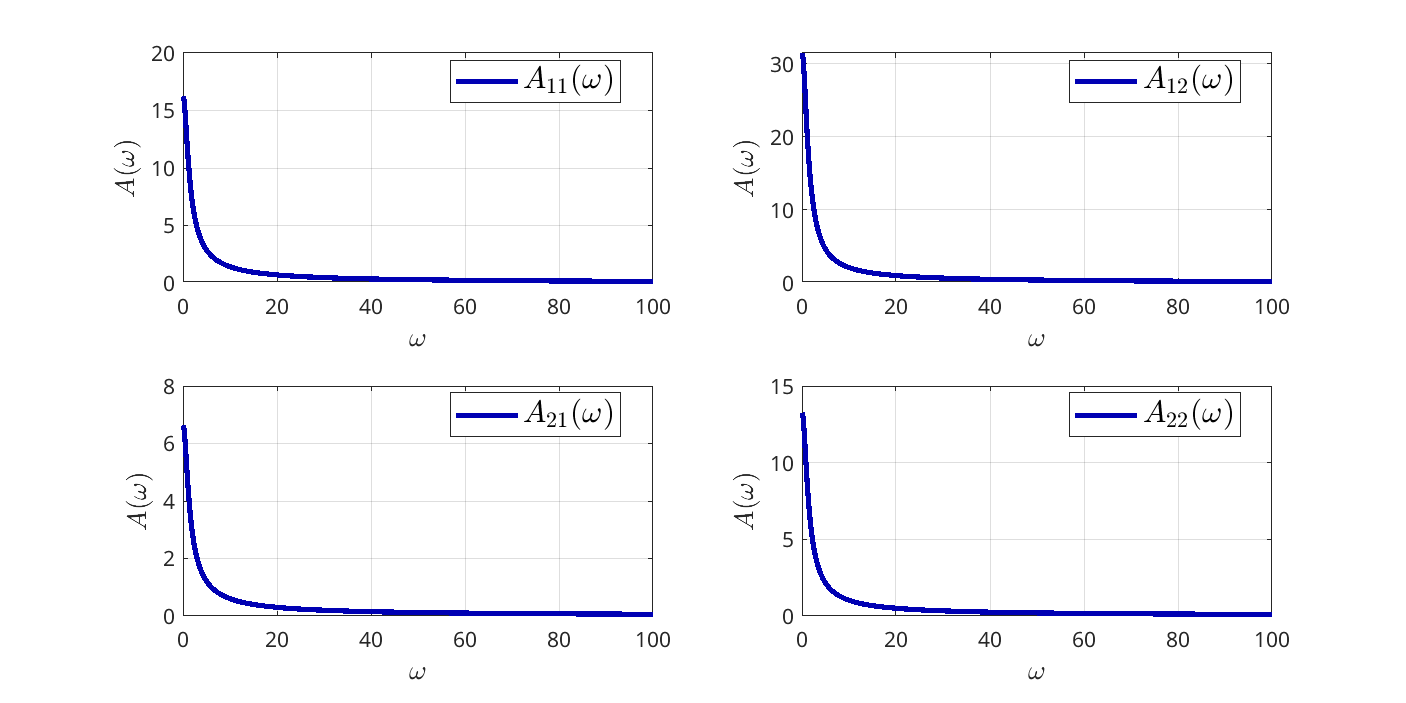
\includegraphics[width=1\textwidth]{../../report/images/task1/ach.png}
		\caption{АЧХ}
	\end{figure}
	
	\begin{figure}[H]
		\centering
		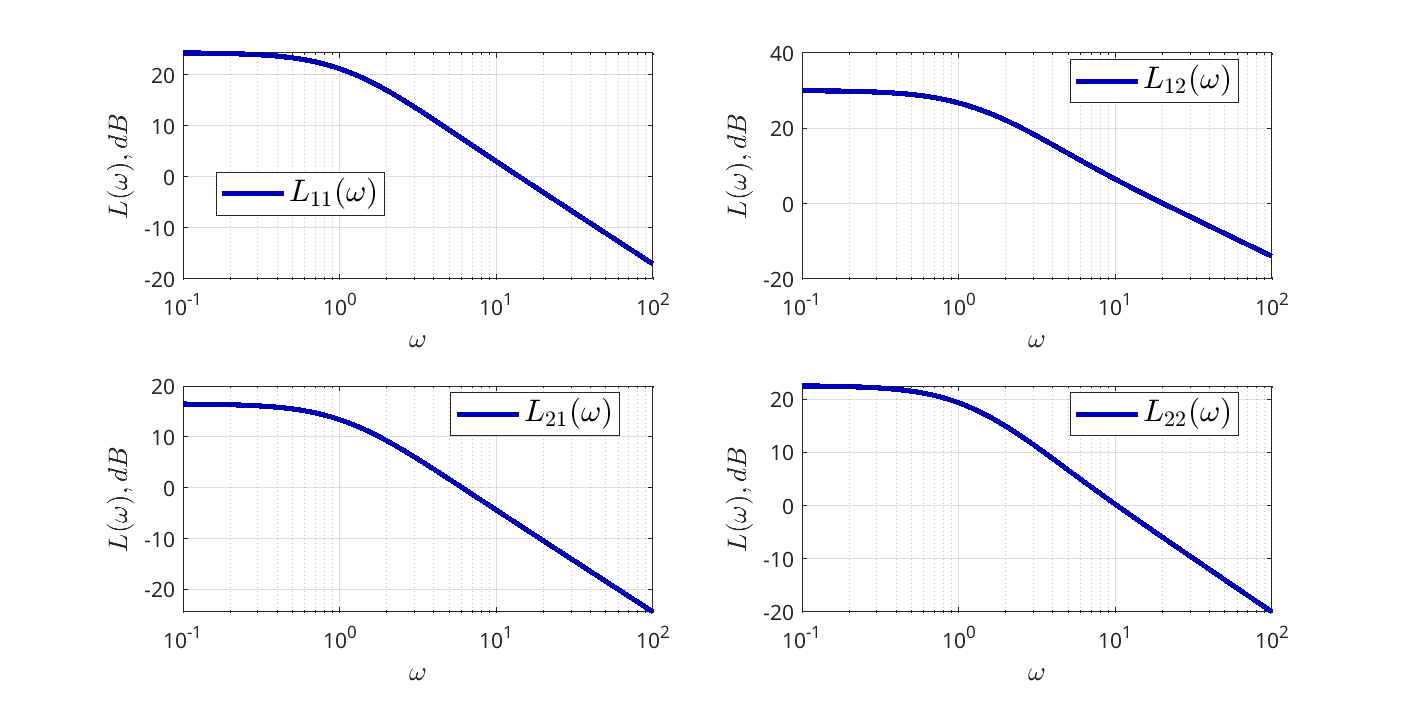
\includegraphics[width=1\textwidth]{../../report/images/task1/lach.png}
		\caption{ЛАЧХ}
	\end{figure}
	
	\begin{figure}[H]
		\centering
		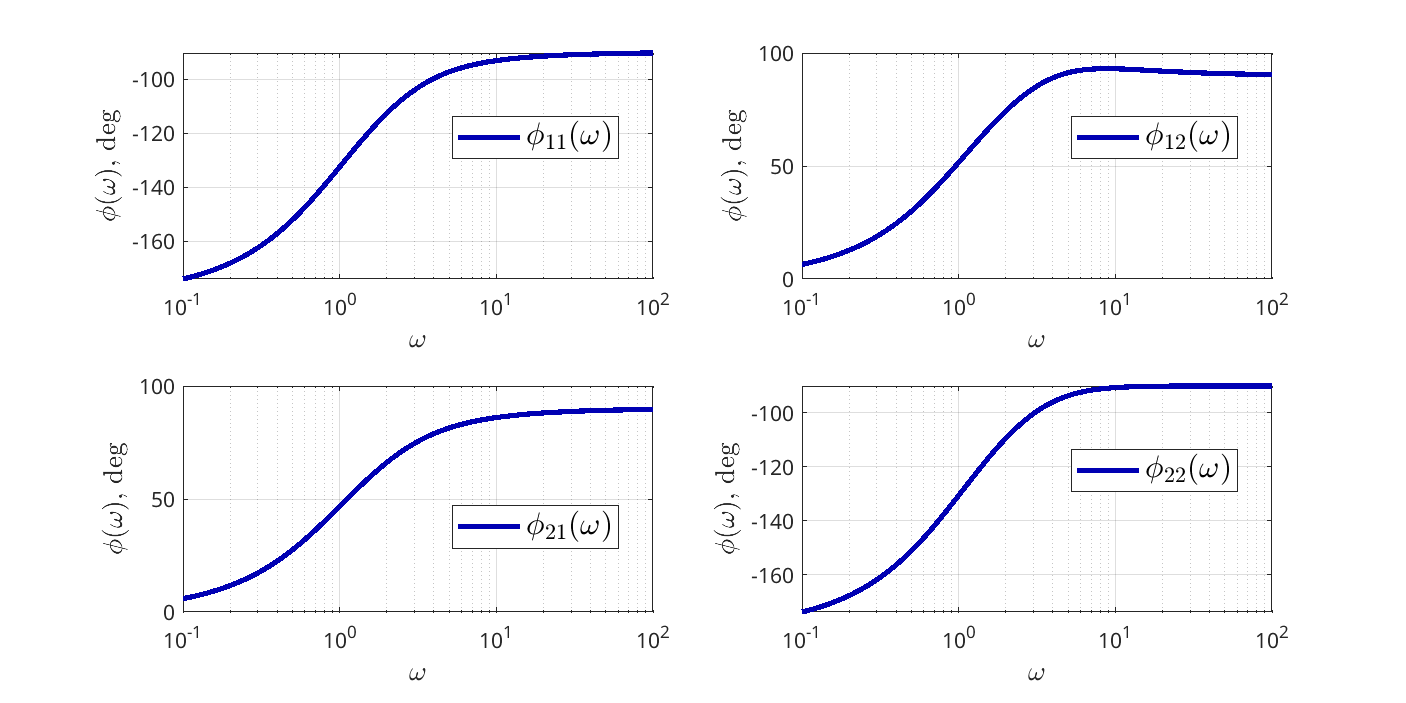
\includegraphics[width=1\textwidth]{../../report/images/task1/fch.png}
		\caption{ФЧХ}
	\end{figure}
	
	\begin{figure}[H]
		\centering
		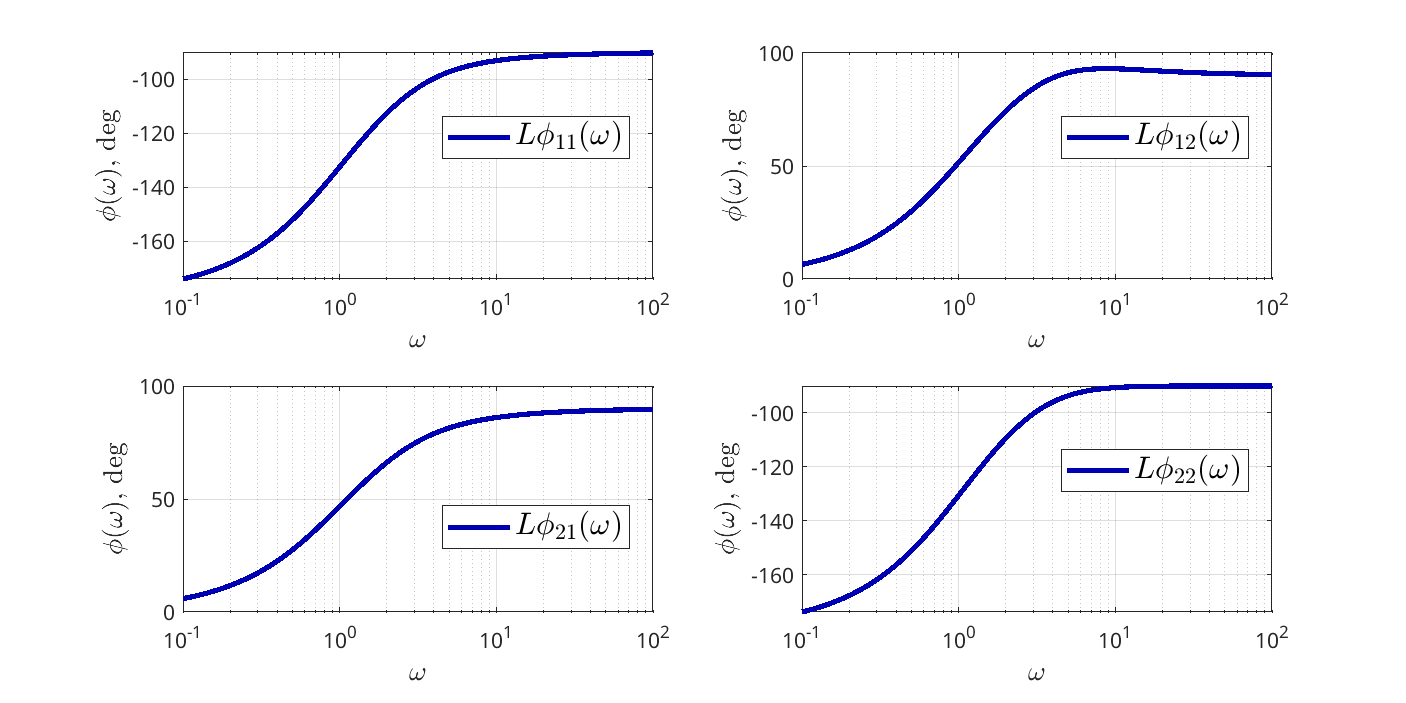
\includegraphics[width=1\textwidth]{../../report/images/task1/lfch.png}
		\caption{ЛФЧХ}
	\end{figure}
	
	\subsection{Выводы}
	
	Система является неустойчивой. Её передаточная матрица имеет полюса, совпадающие с собственными числами матрицы $A$, при этом нули передачи отсутствуют. Система полностью управляема, наблюдаема и управляема по выходу. Временные характеристики экспоненциально возрастают, что подтверждает неустойчивость системы.
	
	
	
	\newpage
	\section{ Синтез следящего управления в условиях внешних возмущений для многоканальной системы}
	
	В соответствии с вариантом необходимо рассмотреть многоканальную систему
	
	\[
	\begin{cases}
		\dot{x} = Ax + Bu + B_f f_1 \\
		z = C_z x + D_z u - g \\
		y = Cx + Du + D_f f_2
	\end{cases}
	\qquad
	x(0) = \begin{bmatrix} 1 & 1 \end{bmatrix}^T
	\]
	
	Матрицы системы
	
	\[
	A = \begin{bmatrix}
		0 & 1 \\
		-3 & 4
	\end{bmatrix}
	\quad
	B = \begin{bmatrix}
		3 & -5 \\
		2 & 0
	\end{bmatrix}
	\quad
	C = \begin{bmatrix}
		4 & 1 \\
		-2 & 0
	\end{bmatrix}
	\quad
	D = \begin{bmatrix}
		2 & 0 \\
		0 & -3
	\end{bmatrix}
	\]
	
	\[
	B_f = \begin{bmatrix}
		3 & 1 \\
		2 & 0
	\end{bmatrix}
	\quad
	D_f = \begin{bmatrix}
		-1 & 0 \\
		0 & 1
	\end{bmatrix}
	\quad
	C_z = \begin{bmatrix}
		3 & 1 \\
		2 & 0
	\end{bmatrix}
	\quad
	D_z = \begin{bmatrix}
		-2 & 0 \\
		0 & 1
	\end{bmatrix}
	\]
	
	Внешние воздействия
	
	\[
	g(t) = \begin{bmatrix}
		4\cos(9t) \\
		3\sin(9t)
	\end{bmatrix}\quad
	f_1(t) = \begin{bmatrix}
		5\sin(2t) \\
		5\cos(4t)
	\end{bmatrix}
	\quad
	f_2(t) = \begin{bmatrix}
		3\cos(4t) \\
		\sin(2t)
	\end{bmatrix}
	\]
	
	Доступны к измерению только $y(t)$ и $g(t)$.\\
	
	Требуется:
	
	\begin{enumerate}
		\item Исследовать систему на управляемость, наблюдаемость, стабилизируемость, обнаруживаемость и управляемость по выходу.
		
		\item Составить передаточные матрицы $W_{yu}(s)$ и $W_{zu}(s)$, проверить их на вырожденность.
		
		\item Построить генератор внешних воздействий, найти $\Gamma_w$, $w(0)$, $Y_g$, $Y_1$, $Y_2$.
		
		\item Построить схему моделирования замкнутой системы с регулятором $u = K\hat{x} + K_w\hat{w}$.
		
		\item Синтезировать матрицы $K$ и $K_w$, проверив условия существования решений.
		
		\item Выполнить моделирование, построить графики $u(t)$, $f_1(t)$, $f_2(t)$, $g(t)$, $y(t)$, $z(t)$, $x(t)$, $w(t)$ и ошибок оценивания.
		
		\item Сделать выводы.
	\end{enumerate}
	
	\hrule \newpage
	
	\subsection{Анализ системы}
	
	Исследую систему по пройденным на курсе критериям.
	
	
	\begin{enumerate}
		\item Построю матрицу управляемости (листинг~\ref{lst:Co1}):
		
		\[
		\mathcal{C} = \begin{bmatrix} B & AB \end{bmatrix} = 
		\begin{bmatrix}
			3 & -5 & 2 & 0 \\
			2 & 0 & -1 & 15
		\end{bmatrix}
		\]
		
		\[
		\text{rank}(\mathcal{C}) = 2
		\]
		
		Следовательно, система полностью управляема по состоянию, а значит  стабилизируема.
		
		
		\item Матрица наблюдаемости (листинг~\ref{lst:Ob1}):
		
		\[
		\mathcal{O} = \begin{bmatrix} C \\ CA \end{bmatrix} = 
		\begin{bmatrix}
			4 & 1 \\
			-2 & 0 \\
			-3 & 8 \\
			0 & -2
		\end{bmatrix}
		\]
		
		\[
		\text{rank}(\mathcal{O}) = 2
		\]
		
		Следовательно, система полностью наблюдаема, а значит, и обнаруживаема.
		
		\item Матрица управляемости по выходу $y(t)$ (листинг~\ref{lst:Co_out_y2}):
		
		\[
		\mathcal{C}_{y} = \begin{bmatrix} CB & CAB & D \end{bmatrix} = 
		\begin{bmatrix}
			14 & -20 & 7 & 15 & 2 & 0 \\
			-6 & 10 & -4 & 0 & 0 & -3
		\end{bmatrix}
		\]
		
		\[
		\text{rank}(\mathcal{C}_{y}) = 2
		\]
		
		Следовательно, система управляема по выходу $y(t)$.
		
		\item Матрица управляемости по виртуальному выходу $z(t)$ (листинг~\ref{lst:Co_out_z2}):
		
		\[
		\mathcal{C}_{z} = \begin{bmatrix} CB & CAB & D_z \end{bmatrix} = 
		\begin{bmatrix}
			11  & -15   &  5   & 15   & -2   &  0\\
			6   &-10    & 4   &  0  &   0   &  1\\
		\end{bmatrix}
		\]
		
		\[
		\text{rank}(\mathcal{C}_{z}) = 2
		\]
		
		Следовательно, система управляема по выходу $z(t)$.
		

	\end{enumerate}
	
	\subsection{Передаточные матрицы}
	
	\begin{enumerate}
		
		\item Передаточная матрица от управления $u(t)$ к выходу $y(t)$ (листинг~\ref{lst:W_yu}):
		\[
		W_{u \rightarrow y}(s) = C(sI - A)^{-1}B + D =
		\frac{1}{s^2 - 4s + 3}
		\begin{bmatrix}
			2s^2 + 6s - 43 & -20s + 95 \\
			-6s + 20 & -3s^2 + 14s - 1
		\end{bmatrix}
		\]
		
		\item Передаточная матрица от управления \(u(t)\) к виртуальному выходу \(z(t)\) (листинг~\ref{lst:W_zu}):
		\[
		W_{u \rightarrow z}(s) = C_z(sI - A)^{-1}B + D_z =
		\frac{1}{s^2 - 4s + 3}
		\begin{bmatrix}
			-2s^2 + 19s - 45 & -15s + 75 \\
			6s - 20 & s^2 - 4s - 7
		\end{bmatrix}
		\]
		
	\end{enumerate}
	
	\(\text{rank}\,W_{u \to y}(s) = \text{rank}\,W_{u \to z}(s) = 2 = n\), где \(n\) --- порядок системы, следовательно, передаточные матрицы невырождены.
	
	
	\subsection{Генератор внешних воздействий}
	
	Для сигналов $f_1(t)$, $f_2(t)$ и $g(t)$ выберу генератор с частотами $\omega_1 = 2$, $\omega_2 = 4$, $\omega_3 = 9$.
	
	Матрица генератора:
	
	\[
	\Gamma_w =
	\begin{bmatrix}
		0 & 2 & 0 & 0 & 0 & 0 \\
		-2 & 0 & 0 & 0 & 0 & 0 \\
		0 & 0 & 0 & 4 & 0 & 0 \\
		0 & 0 & -4 & 0 & 0 & 0 \\
		0 & 0 & 0 & 0 & 0 & 9 \\
		0 & 0 & 0 & 0 & -9 & 0
	\end{bmatrix} \qquad
	w(0) = 
	\begin{bmatrix}
		1 \\ 0 \\ 1 \\ 0 \\ 1 \\ 0
	\end{bmatrix}
	\]
	
	Для $g(t)$:
	
	\[
	g(t) = 
	\begin{bmatrix}
		4\cos 9t \\
		3\sin 9t
	\end{bmatrix}
	\qquad \Longrightarrow \qquad Y_g = 
	\begin{bmatrix}
		0 & 0 & 0 & 0 & 4 & 0 \\
		0 & 0 & 0 & 0 & 0 & -3
	\end{bmatrix}
	\]
	
	Для $f_1(t)$:
	
	\[
	f_1(t) = 
	\begin{bmatrix}
		5\sin 2t \\
		5\cos 4t
	\end{bmatrix}
	\qquad \Longrightarrow \qquad
	Y_1 = 
	\begin{bmatrix}
		0 & -5 & 0 & 0 & 0 & 0 \\
		0 & 0 & 5 & 0 & 0 & 0
	\end{bmatrix}
	\]
	
	Для $f_2(t)$:
	
	\[
	f_2(t) = 
	\begin{bmatrix}
		3\cos 4t \\
		\sin 2t
	\end{bmatrix}
	\qquad \Longrightarrow \qquad
	Y_2 = 
	\begin{bmatrix}
		0 & 0 & 3 & 0 & 0 & 0 \\
		0 & -1 & 0 & 0 & 0 & 0
	\end{bmatrix}
	\]
	
	\subsection{Синтез матрицы \(K\)}
	

Выберу желаемые полюса замкнутой системы $\lambda_i^*$ и запишу матрицу желаемой динамики:
\[
\lambda_1^* = -4 \quad \lambda_2^* = -5 \qquad
\Gamma = \begin{bmatrix} -4 & 0 \\ 0 & -5 \end{bmatrix}
\]

Для синтеза матрицы $K$ необходимо решить матричное уравнение Сильвестра:
\[
AP - P\Gamma = BY
\]
Предварительно проверю условия существования единственного невырожденного решения:

\begin{enumerate}
	\item Непересечение спектров:
	\[
	\sigma(A) = \{1, 3\} \cap \sigma(\Gamma) = \{-4, -5\} = \varnothing
	\]
	
	\item Управляемость пары $(A, B)$:
	\[
	\mathcal{C} = \begin{bmatrix} B & AB \end{bmatrix} = 
	\begin{bmatrix}
		3 & -5 & 2 & 0 \\
		2 & 0 & -1 & 15
	\end{bmatrix}\qquad \operatorname{rank}\mathcal{C} = 2
	\]
	
	\item Наблюдаемость пары $(Y, \Gamma)$:
	Выберу вспомогательную матрицу $Y = \begin{bmatrix} 1 & 1 \\ 1 & 1 \end{bmatrix}$. Матрица наблюдаемости:
	\[
	\mathcal{O}_{Y,\Gamma} = \begin{bmatrix} Y \\ Y\Gamma \end{bmatrix} = 
	\begin{bmatrix}
		1 & 1 \\ 1 & 1 \\ -4 & -5 \\ -4 & -5
	\end{bmatrix} \qquad \operatorname{rank}\mathcal{O}_{Y,\Gamma} = 2
	\]
\end{enumerate}

Все необходимые условия выполнены. Решая уравнение Сильвестра (листинг~\ref{lst:sylv2}), получаю матрицу $P$:
\[
P = \begin{bmatrix} -0.5143 & -0.4167 \\ 0.0571 & 0.0833 \end{bmatrix}
\]

Матрица регулятора:
\[
K = -YP^{-1} = \begin{bmatrix} 1.3750 & -5.1250 \\ 1.3750 & -5.1250 \end{bmatrix}
\]

\subsection{Синтез матрицы \(K_w\)}

Для синтеза компенсирующей компоненты регулятора составлю систему матричных уравнений Франкиса--Дэвисона:
\[
\begin{cases}
	P \Gamma_w - (A + BK)P - B_f Y_1 = B K_w \\
	(C_z + D_z K)P + D_z K_w = Y_g
\end{cases}
\]

Условием существования решения данной системы является выполнение условия полного ранга для каждого собственного числа $\lambda \in \sigma(\Gamma_w)$:
\[
\operatorname{rank}
\begin{bmatrix}
	A + BK - \lambda I & B \\
	C_z + D_z K & D_z
\end{bmatrix}
= 4
\]

Условие выполняется для всех собственных чисел $\Gamma_w$ (листинг~\ref{lst:check_fd}). Решение существует.\\



Найду матрицу $P$, решив соответствующее уравнение Сильвестра, а затем вычислю матрицу $K_w$ (листинг~\ref{lst:kw_synthesis}):

\[
\begin{aligned}
	P &= \begin{bmatrix}
		0.0169 & 0.7395 & -0.3204 & -0.0884 & 0.7650 & -0.6182 \\
		-0.6897 & 1.7241 & 0 & 0 & 0.1887 & 0.3396
	\end{bmatrix} \\[5pt]
	K_w &= \begin{bmatrix}
		-3.8772 & 9.7907 & -0.0401 & -0.0110 & -0.8431 & 1.8331 \\
		-3.5915 & 6.3402 & 1.0815 & 0.2983 & -1.6148 & 0.8271
	\end{bmatrix}
\end{aligned}
\]

	

	
	
\subsection{Синтез наблюдателей}

Для построения наблюдателя сформирую расширенную систему, объединив векторы состояния объекта и генератора возмущений:

\[
x_f = \begin{bmatrix} w \\ x \end{bmatrix}
\]

Матрицы расширенной системы определяются выражениями:

\[
\bar{A} = \begin{bmatrix} \Gamma_w & 0 \\ B_f Y_1 & A \end{bmatrix} \qquad
\bar{B} = \begin{bmatrix} 0 \\ B \end{bmatrix}
\]

Измеряемый вектор включает выход системы и сигнал генератора:

\[
\tilde{y} = \begin{bmatrix} y \\ g \end{bmatrix}
\]

Матрица выхода расширенной системы имеет вид:

\[
\tilde{C} = \begin{bmatrix} D_f Y_2 & C \\ Y_g & 0 \end{bmatrix} \qquad
\tilde{D} = \begin{bmatrix} D \\ 0 \end{bmatrix}
\]

Уравнение наблюдателя полной размерности:

\[
\dot{\hat{x}}_{ext}  = (\bar{A} - L\tilde{C})\hat{x}_{ext}  + (\bar{B} - L\tilde{D})u + L\tilde{y}
\]

Выберу желаемые полюса наблюдателя:

\[
\lambda_{obs} = [-10, -11, -12, -13, -14, -15, -16, -17]^T
\]

Синтезирую матрицу наблюдателя \(L\) методом размещения полюсов для транспонированной пары $(\bar{A}^T, \tilde{C}^T)$ (листинг~\ref{lst:L2}):

\[
L = \begin{bmatrix}
	-8.3364 & -43.8889 & 0 & 0 \\
	24.6276 & 68.6823 & 0 & 0 \\
	35.1074 & 66.2140 & 0 & 0 \\
	-9.5505 & -28.3425 & 0 & 0 \\
	0 & 0 & 4.2500 & -3.0000 \\
	0 & 0 & -2.2500 & -4.0000 \\
	-11.8260 & -53.1320 & 0 & 0 \\
	198.0446 & 422.6576 & 0 & 0
\end{bmatrix}
\]

	
	\subsection{Структурная схема системы}
	
	Структурная схема замкнутой системы представлена на рисунке \ref{fig:scheme}. Регулятор формирует управление $u(t)$ на основе оценок $\hat{x}(t)$ и $\hat{w}(t)$, поступающих от наблюдателя расширенной размерности.
	
	\begin{figure}[H]
		\centering
		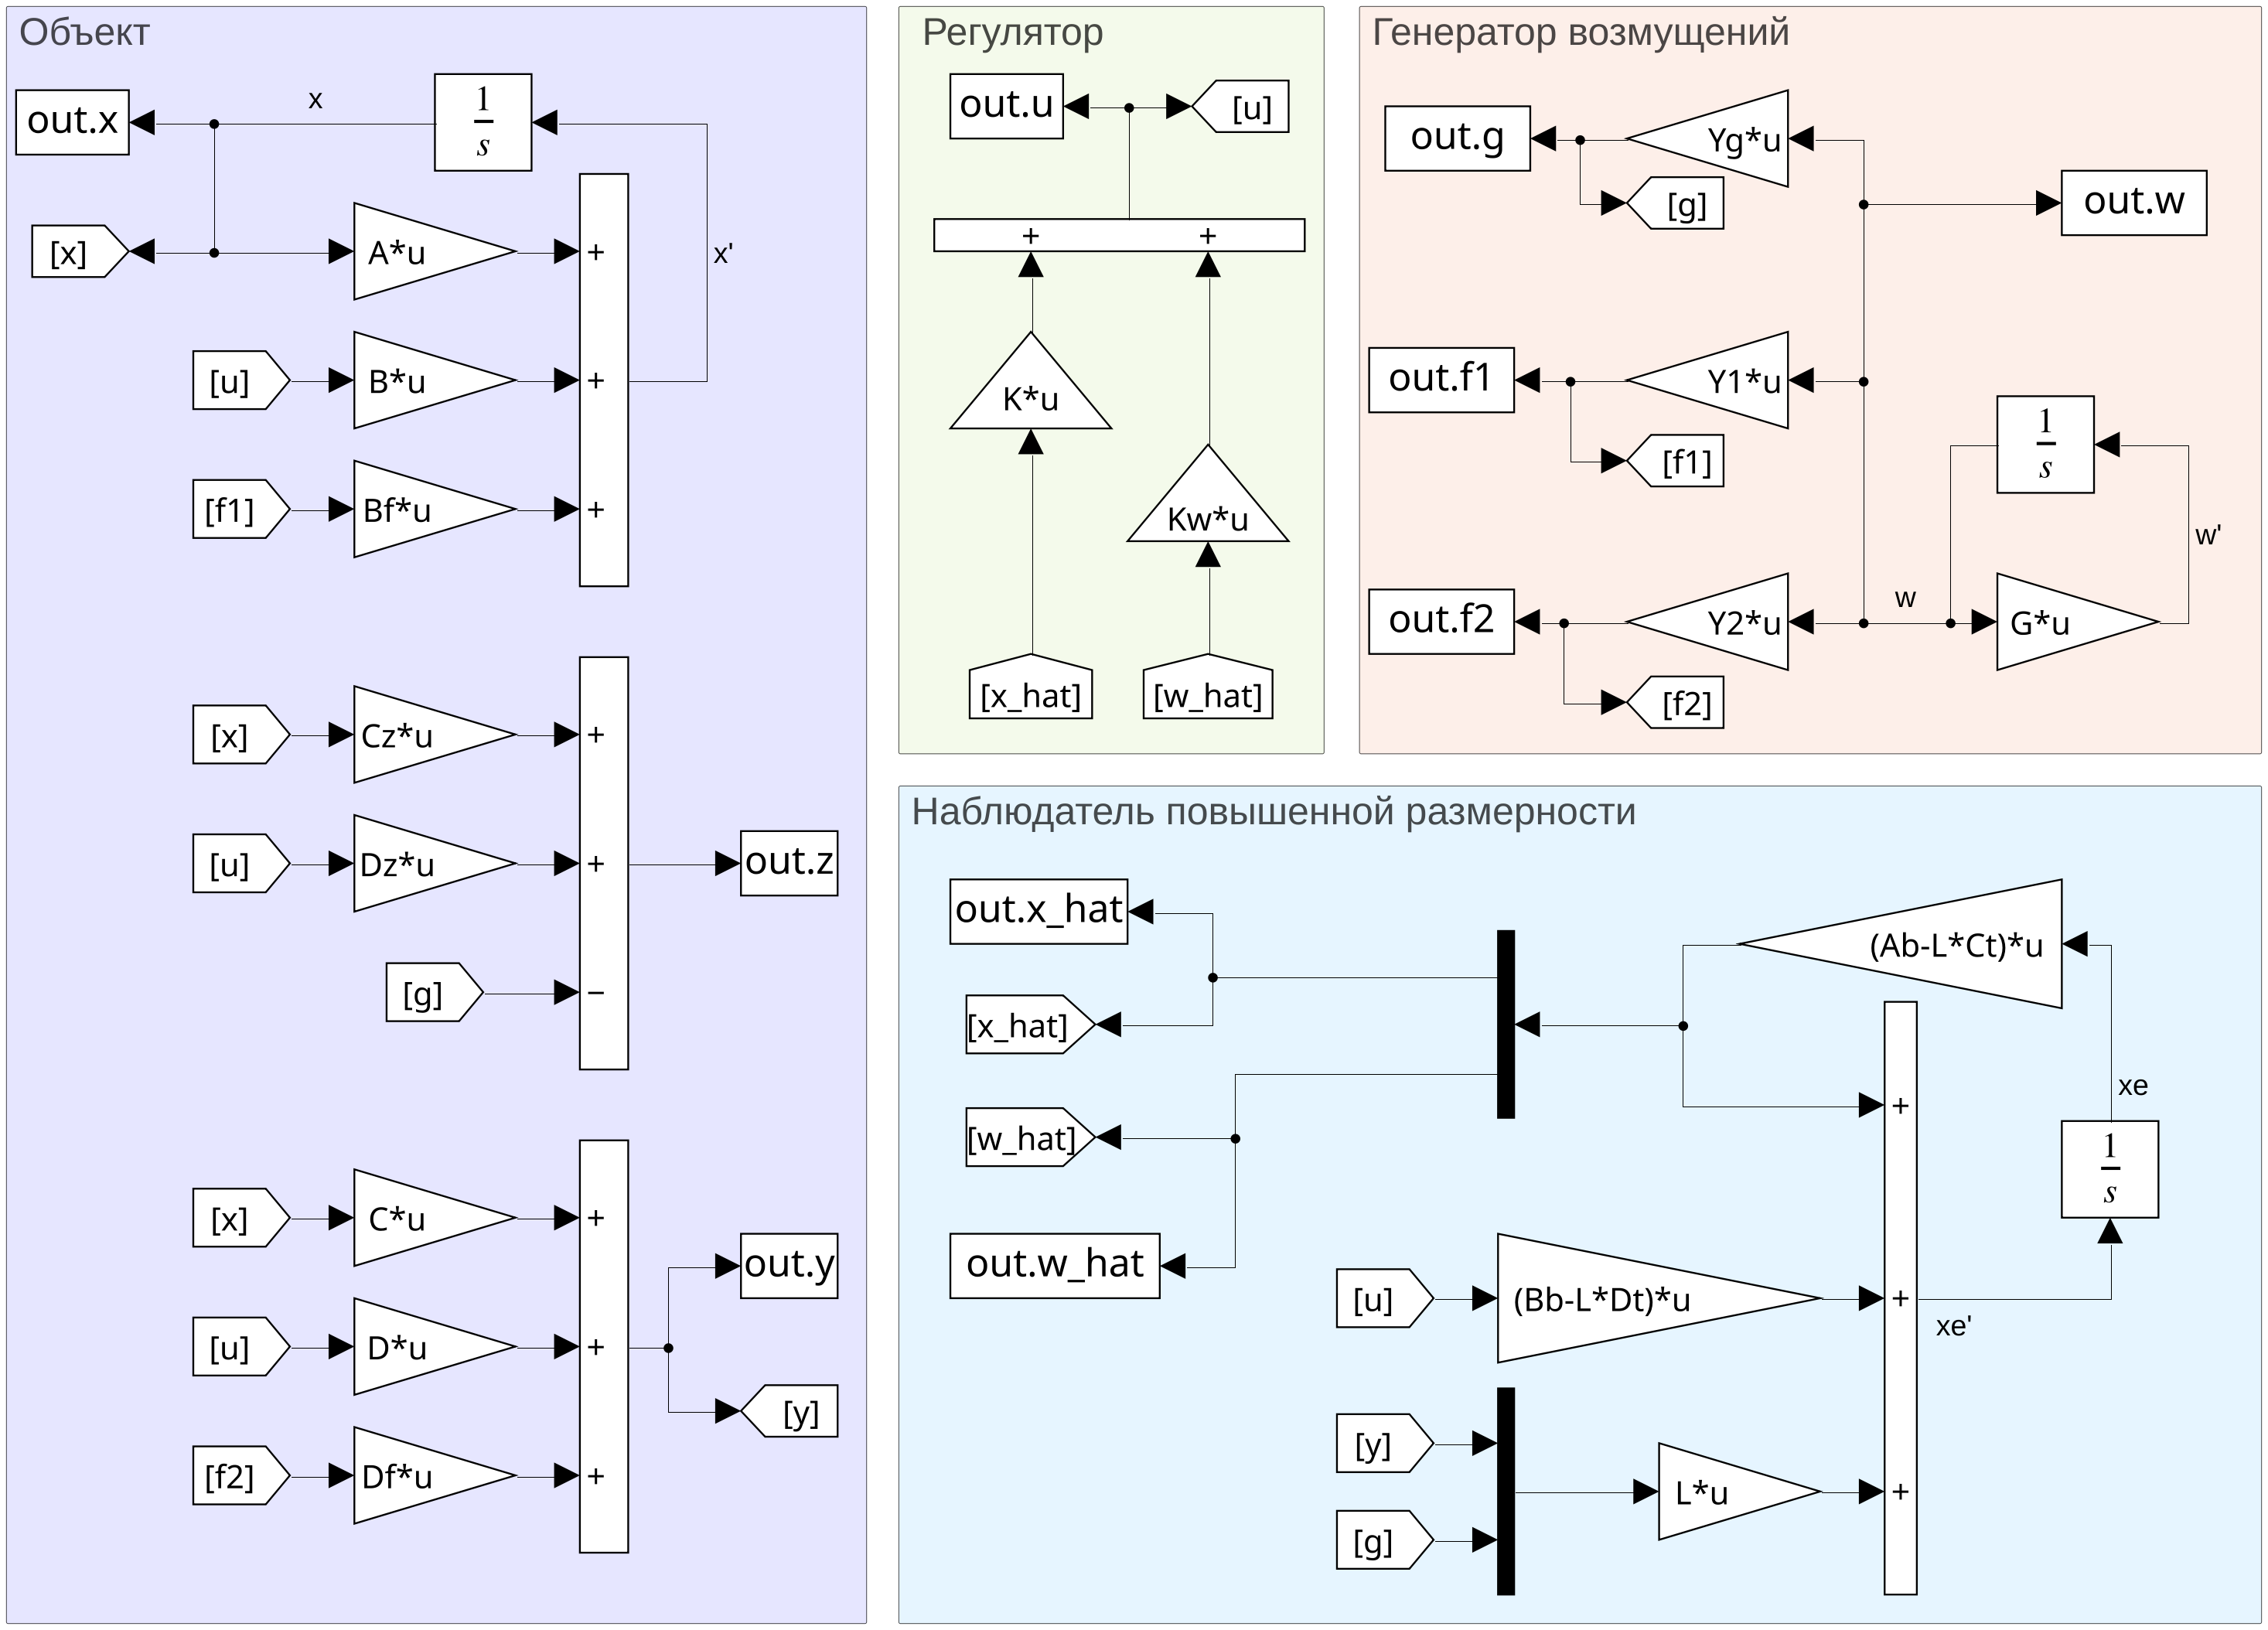
\includegraphics[width=1\textwidth]{../../report/images/task2/closed_observer.png}
		\caption{Структурная схема замкнутой системы}
		\label{fig:scheme}
	\end{figure}
	
	Закон управления имеет вид:
	
	\[
	u = K\hat{x} + K_w\hat{w}
	\]
	
	Наблюдатель расширенной размерности описывается уравнением:
	
	\[
	\dot{\hat{x}}_{ext}  = (\bar{A} - L\tilde{C})\hat{x}_f + (\bar{B} - L\tilde{D})u + L\tilde{y}
	\]
	
	где: 
	\[
	\hat{x}_{ext} = \begin{bmatrix} \hat{w} \\ \hat{x} \end{bmatrix} \qquad
	\tilde{y} = \begin{bmatrix} y \\ g \end{bmatrix}
	\]
	
	
	
	\subsection{Моделирование}
	
	
	
	
	
	
	
	
	
	
	
	\newpage
\section{Приложение}

\subsection*{Задание 1}

\begin{lstlisting}[caption={Инициализация}]
A = [0 1; -3 4];
B = [3 -5; 2 0];
C = [4 1; -2 0];
\end{lstlisting}

\begin{lstlisting}[caption={Собственные числа матрицы \(A\)}, label={lst:A1}]
eig(A)
\end{lstlisting}

\begin{lstlisting}[caption={Передаточная матрица системы}, label={lst:W1}]
syms s
W = simplify(C * inv(s*eye(2) - A) * B)
\end{lstlisting}

\begin{lstlisting}[caption={Определитель передаточной матрицы}, label={lst:detW1}]
detW = simplify(det(W))
\end{lstlisting}

\begin{lstlisting}[caption={Исследование управляемости}, label={lst:Co1}]
Co = ctrb(A, B)
rank(Co) == 2
\end{lstlisting}

\begin{lstlisting}[caption={Исследование наблюдаемости}, label={lst:Ob1}]
Ob = obsv(A, C)
rank(Ob)== 2
\end{lstlisting}
	
	
\begin{lstlisting}[caption={Исследование управляемости по выходу}, label={lst:Co_out1}]
Co_out = [C*B, C*A*B]
\end{lstlisting}	
	
	
\begin{lstlisting}[caption={Весовая характеристика}, label={lst:g1}]
g = simplify(ilaplace(W, s, t))
\end{lstlisting}
	
\begin{lstlisting}[caption={Переходная характеристика}, label={lst:h1}]
h = simplify(ilaplace(W / s, s, t))
\end{lstlisting}	

\begin{lstlisting}[caption={АЧХ}, label={lst:ach1}]
A_ach = simplify(abs(W_jw))
\end{lstlisting}

\begin{lstlisting}[caption={ФЧХ}, label={lst:fch1}]
phi_fch = simplify(angle(W_jw))
\end{lstlisting}

\newpage

\subsection*{Задание 2}

\begin{lstlisting}[caption={Инициализация}]
A = [0 1; -3 4];
B = [3 -5; 2 0];
C = [4 1; -2 0];
D = [2 0; 0 -3];
Bf = [3 1; 2 0];
Df = [-1 0; 0 1];
Cz = [3 1; 2 0];
Dz = [-2 0; 0 1];
x0 = [1; 1];
\end{lstlisting}

\begin{lstlisting}[caption={Исследование управляемости по выходу}, label={lst:Co_out_y2}]
Co_out_y = [C*B, C*A*B, D];
\end{lstlisting}	

	
\begin{lstlisting}[caption={Исследование управляемости по виртуальному выходу}, label={lst:Co_out_z2}]
Co_out_z = [Cz*B, Cz*A*B, Dz]
\end{lstlisting}

\begin{lstlisting}[caption={Передаточная матрица к выходу}, label={lst:W_yu}]
W_yu = simplify(C * inv(s*eye(2) - A) * B + D)
\end{lstlisting}

\begin{lstlisting}[caption={Передаточная матрица к виртуальному выходу}, label={lst:W_zu}]
W_zu = simplify(C * inv(s*eye(2) - A) * B + Dz)
\end{lstlisting}

\begin{lstlisting}[caption={Матрица регулятора \(K\)}, label={lst:sylv2}]
Gamma = [-4  0; 0 -5]
Y = [1 1; 1 1]
P = sylvester(A, -Gamma, B*Y)
K = -Y * inv(P)
\end{lstlisting}


\begin{lstlisting}[caption={Проверка условий существования решения уравнений Франкиса--Дэвисона}, label={lst:check_fd}]
Acl = A + B*K;
F = Cz + Dz*K;
for lambda = eig(G).'
	M = [Acl - lambda*eye(n), B; F, Dz];
	fprintf('lambda = %g%+gi, rank = %d\n', ...
	real(lambda), imag(lambda), rank(M));
end
\end{lstlisting}

\begin{lstlisting}[caption={Синтез матрицы \(K_w\)}, label={lst:kw_synthesis}]
Dz_inv = inv(Dz); 
A_eq = -Acl + B * Dz_inv * F;
B_eq = Bf*Y1 + B * Dz_inv * Yg;
P = sylvester(A_eq, G, B_eq);
Kw = Dz_inv * (Yg - F*P);
\end{lstlisting}
	
\begin{lstlisting}[caption={Синтез матрицы \(L\)}, label={lst:L2}]
lambda_obs = [-10; -11; -12; -13; -14; -15; -16; -17]
L = place(Ab', Ct', lambda_obs)'
\end{lstlisting}
	
	
	

	
\end{document}